\documentclass{article}
\usepackage{graphicx}
\usepackage{float}
\usepackage{booktabs}
\usepackage[utf8]{inputenc}
\usepackage{listings}
\usepackage{xcolor}
\usepackage{amsmath}
\lstset{
    language=Python,
    backgroundcolor=\color{white}, % Set background color for code
    basicstyle=\ttfamily, % Set font for code
    keywordstyle=\color{blue}, % Color for keywords
    commentstyle=\color{green}, % Color for comments
    stringstyle=\color{red}, % Color for strings
    showstringspaces=false, % Don't show spaces in strings
    breaklines=true, % Break long lines
    frame=single % Add frame around code
}     
\usepackage{tocloft}
\usepackage[norsk]{babel}
\usepackage[a4paper, left=20mm, right=20mm, top=25mm, bottom=25mm]{geometry}
\usepackage[linkcolor=black, urlcolor=black, citecolor=black, hidelinks]{hyperref}

\begin{document}
\title{Andel BK74 blant tungtrafikken over\\BWIM sensorene på Sørbryn og Tangensvingen}
\author{}
\maketitle
% \tableofcontents

\newpage


Intensjonen med dette arbeidet var å sette opp en oversikt over andelen BK74 blant tungtrafikken som har gått
over de 2 BWIM sensorene benyttet i tømmertransportprosjektet. Dette vil si sensorene på Sørbryn og Tangensvingen.
For å overkomme problematikken rundt at BWIM sensorene kun er i drift i begrensede perioder, tok jeg utgangspunkt i
data samlet inn fra deres respektivt nærmeste kontinuerlige trafikktellepunkter. Dette vil si svartelva for Sørbryn,
og Tangensvingen vest for Tangensvingen. Ettersom man er avhengig av å finne antallet BK74 passeringer over BWIM sensorene
for å finne andelen av den totale tungtrafikken, mens dataen fra prøveordningen kommer som tids-merkede koordinatpunkter, er det
her blitt benyttet et område for å telle registreringer for stedene man er interessert i å telle passeringer for. Områdene er utformet slik
at all trafikk som kjører gjennom området er nødt til å passere over stedet man teller passeringer for.
Figur \ref{fig:heatmap} viser et eksempel på logginger fra prøveordningen, mens
Figur \ref{fig:tangensvingen_bru_tangensvingen_vest} viser området som er benyttet for å telle passeringer over Tangensvingen bru,
med hensyn på "utstikkerne" som hadde blitt inkludert dersom man strakk området lenger.

\begin{figure}[H]
    \centering
    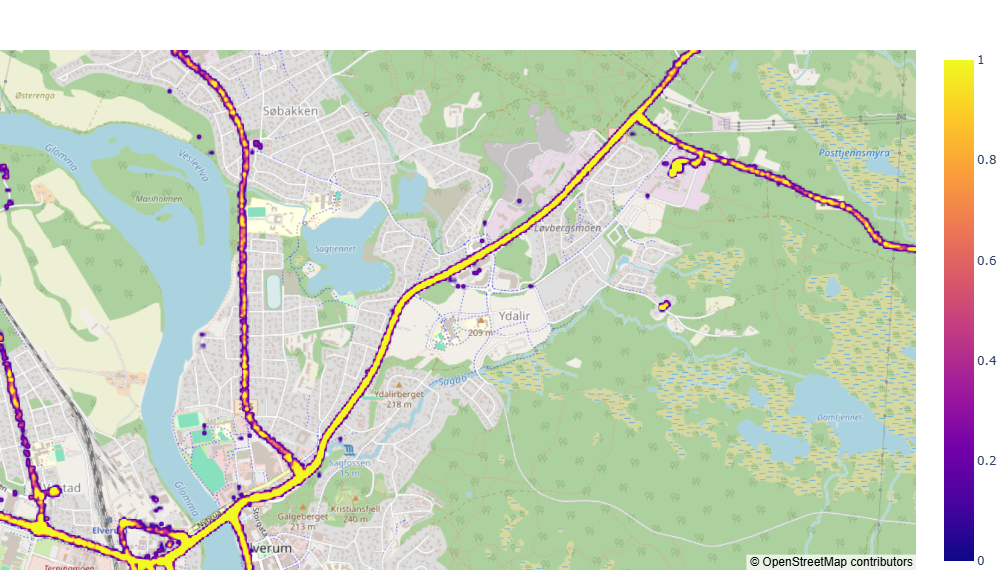
\includegraphics[width=1\textwidth]{./figures/heatmap.png}
    \caption{Eksempel på trafikk fra prøveordningen}
    \label{fig:heatmap}
\end{figure}


\begin{figure}[H]
    \centering
    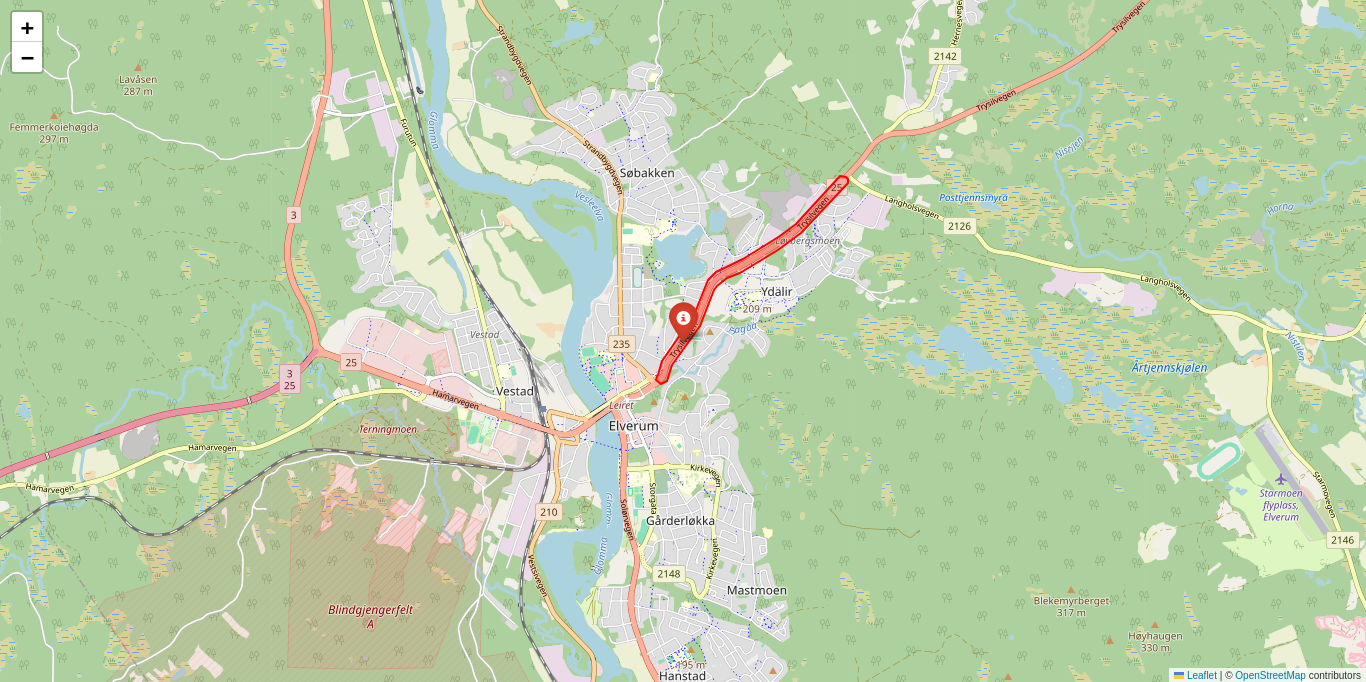
\includegraphics[width=1\textwidth]{./figures/tangensvingen_bru_tangensvingen_vest.png}
    \caption{Området benyttet til å finne passeringer av tangensvingen bru}
    \label{fig:tangensvingen_bru_tangensvingen_vest}
\end{figure}

Ved å benytte fremgangsmåten beskrevet i vedlegget under, satt jeg igjen med en god del registreringer.
Disse registreringene er vist i Figur \ref{fig:tangensvingen_all_markers}, og oppsummert i Figur \ref{fig:markerclusters}.

\begin{figure}[H]
    \centering
    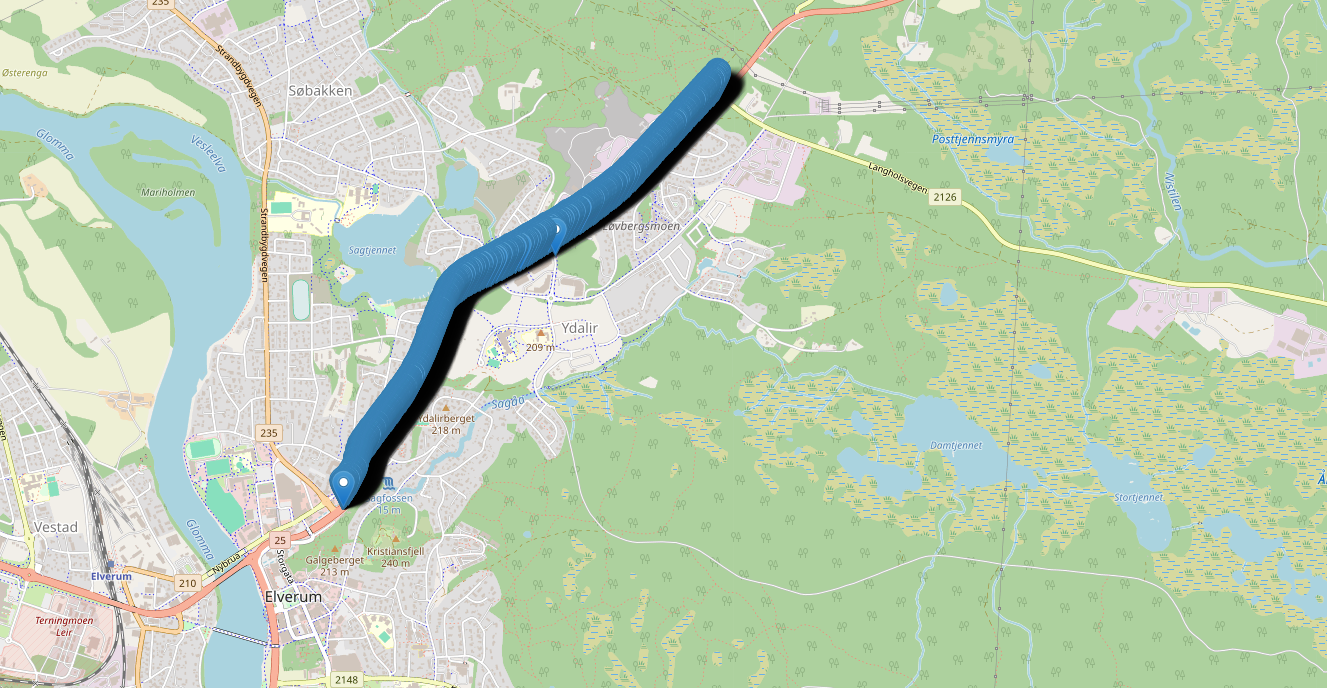
\includegraphics[width=1\textwidth]{./figures/tangensvingen_all_markers.png}
    \caption{Alle registreringer markert som gyldige}
    \label{fig:tangensvingen_all_markers}
\end{figure}

\begin{figure}[H]
    \centering
    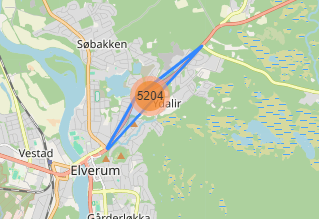
\includegraphics[width=1\textwidth]{./figures/markerclusters.png}
    \caption{Oppsumering av registreringer markert som gyldige}
    \label{fig:markerclusters}
\end{figure}

Som Figur \ref{fig:markerclusters} viser, er det 5204 registreringer (sum alle år, alle ekvipasjer) som er regnet som gyldige passeringer.
Imidlertid viser trafikktellepunktene fra veidata at det skal ha vært 612 registrerte passeringer av kjøretøy over 16 meter i det samme tidsspennet.
Ettersom BK74 er godt over dette, så kan dette tyde på at det er forhold her som ikke er helt klare
\end{document}
